\chapter{Regressione}
Definiamo il compito di regressione in termini di come un algoritmo elabora un esempio
di input e produce un valore (o vettore) reale di output. Formalmente, vogliamo
apprendere una funzione


\[
h_\vartheta:\ \mathbb{R}^{d_1}\rightarrow \mathbb{R}^{d_2},\qquad d_1\ge 1,\ d_2\ge 1,
\]
a partire da un dataset supervisionato
\[
D=\{(x^{(i)},y^{(i)})\}_{i=1}^m,\qquad x^{(i)}\in\mathbb{R}^{d_1},\ y^{(i)}\in\mathbb{R}^{d_2}.
\]

\noindent
In altre parole, individuare una funzione nello spazio dei dati, passante per tutti i valori del dataset in input, e presumibilmente capace di predirre il valore associato ai dati di testing. Permette quindi di \textbf{stabilire relazioni tra i dati}, \textbf{individuare trend} e fare predizioni.

\section{Ingredienti del task}
\begin{itemize}
  \item \textbf{Task}: predire valori reali a partire da input reali.
  \item \textbf{Modello}: ipotesi parametrica \(h_\vartheta\) che mappa input in output.
  \item \textbf{Dati}: coppie etichettate \((x^{(i)},y^{(i)})\).
  \item \textbf{Algoritmo di learning}: metodo per stimare \(\vartheta\) (ottimizzazione).
  \item \textbf{Funzione di loss}: misura lo scarto tra predizioni e target.
  \item \textbf{Valutazione}: metriche su validation/test per giudicare il modello.
\end{itemize}

\subsection{Tipi di regressione}

\begin{enumerate}
	\item \textbf{Regressione lineare}, $h_\vartheta : \mathbb{R} \to \mathbb{R}$, da spazio a una dimensione a una dimensione.
	\item \textbf{Multiple regression}, $h_\vartheta : \mathbb{R}^{d_1} \to \mathbb{R}$, $d_1 > 1$, con $d_1$ features di input e un output.
	\item \textbf{Multivariate regression}, $h_\vartheta : \mathbb{R}^{d_1} \to \mathbb{R}^{d_2}$, $d_1, d_2 > 1$, con $d_1$ features di input e $d_2$ output. Un modello di multivariate regression, viene allenato come un modello di multiple regression su ciascuno degli output.
\end{enumerate} 
\section{Regressione lineare semplice}
Nel caso \(d_1=d_2=1\) modelliamo la relazione tra un singolo ingresso \(x\in\mathbb{R}\) e
un'uscita reale \(y\in\mathbb{R}\) con una retta:
\[
h_\vartheta(x)=\vartheta_0+\vartheta_1\,x,
\]
dove \(\vartheta_0\) è l'intercetta e \(\vartheta_1\) la pendenza. ``Imparare'' significa scegliere
\(\vartheta=(\vartheta_0,\vartheta_1)\) in modo che le predizioni siano vicine ai corrispondenti target.

\subsection{Funzione di loss}
Misuriamo la qualità della retta con l'errore medio quadratico (MSE):
\[
J(\vartheta)=\frac{1}{2m}\sum_{i=1}^{m}\big(h_\vartheta(x^{(i)})-y^{(i)}\big)^2.
\]
Il fattore \(1/2\) è una costante di comodo che semplifica le derivate; il quadrato rende
positivi tutti i contributi ed enfatizza gli errori grandi. In regressione lineare \(J\) è
convessa rispetto ai parametri, quindi il minimo è unico (se c'è variabilità negli \(x^{(i)}\)). Otteniamo un grafico a tazza.
\section{Regressione lineare multipla}
Estendiamo al caso con più variabili in ingresso. Dato il vettore
\(x=(x_1,\dots,x_n)\), usiamo un parametro per ogni dimensione più il bias:
\[
f(x)=\vartheta_0+\vartheta_1x_1+\vartheta_2x_2+\cdots+\vartheta_n x_n .
\]
Per semplicità poniamo \(x_0=1\) e definiamo il vettore esteso
\(
x=(x_0,x_1,\dots,x_n)^\top
\);
allora
\[
f(x)=\sum_{i=0}^n \vartheta_i x_i \;=\; \boldsymbol{\vartheta}^\top x.
\]
Questo modello è, in sostanza, un \emph{percettrone senza soglia}: la combinazione lineare
\(\boldsymbol{\vartheta}^\top x\) è l'uscita continua del regressore.

\section{Feature scaling}
Per far funzionare bene (e in fretta) la discesa del gradiente, le feature vanno portate
su scale simili. Due opzioni comuni:
\[
\text{z-scoring:}\quad x_j\leftarrow\frac{x_j-\mu_j}{\sigma_j},
\qquad
\text{min--max:}\quad x_j\leftarrow\frac{x_j-x_j^{\min}}{x_j^{\max}-x_j^{\min}}.
\]
Le statistiche \((\mu_j,\sigma_j,x_j^{\min},x_j^{\max})\) si calcolano solo sul training e
si riusano (senza ricalcolarle) su validation/test, per evitare data leakage.

\section{Algoritmo di discesa del gradiente}
L’obiettivo è scegliere \(\vartheta\) che minimizza \(J(\vartheta)\) funzione di loss. La \emph{discesa del gradiente}
è un metodo iterativo che aggiorna i parametri nella direzione di massima diminuzione di \(J\).
Nel prossimo esempio a due parametri ($\vartheta_0, \vartheta_1$), supporremo l'intercetta $\vartheta_0 = 0$.

\subsection{Idea dell'algoritmo}
Partiremo da dei valori casuali dei parametri, in questo caso $\vartheta_1$, in quanto $\vartheta_0$ è già fissata a 0 per semplicità.
Osserveremo il coefficiente angolare della retta tangente alla funzione di loss, ossia la sua derivata. Quando questa è:
\begin{itemize}
	\item negativa, incrementare il valore.
	\item positiva, decrementare il valore,
\end{itemize}

Il numero di iterazioni da ripetere dipende dalla convergenza che si vuole ottenere.

\subsection{Algoritmo generale}
Sia \(X\in\mathbb{R}^{m\times(n+1)}\) la design matrix con prima colonna di \(1\),
\(y\in\mathbb{R}^{m}\) il vettore dei target e \(\hat y=X\vartheta\) le predizioni. La loss è
\[
J(\vartheta)=\frac{1}{2m}\|X\vartheta-y\|_2^2,\qquad
\nabla_\vartheta J(\vartheta)=\frac{1}{m}X^\top(X\vartheta-y).
\]

\paragraph{Pseudocodice.}
\begin{enumerate}
  \item \textbf{Inizializza} in modo casuale: \(\vartheta^{(0)}=(\vartheta_0,\ldots,\vartheta_n)^\top\).
  \item \textbf{Calcola le derivate parziali}:
  \[
  \frac{\partial J(\vartheta)}{\partial \vartheta_j}
  =\frac{1}{m}\sum_{i=1}^m\big(\vartheta^\top \tilde x^{(i)}-y^{(i)}\big)\,\tilde x^{(i)}_j,\qquad j=0,\ldots,n,
  \]
  dove \(\tilde x^{(i)}=(1,x^{(i)}_1,\ldots,x^{(i)}_n)^\top\).
  \item \textbf{Aggiorna} i parametri (passo di ampiezza \(\alpha>0\)):
  \[
  \vartheta_j \leftarrow \vartheta_j - \alpha\,\frac{\partial J(\vartheta)}{\partial \vartheta_j},
  \qquad j=0,\ldots,n.
  \]
  \item \textbf{Ripeti} i passi 2–3 finché non è soddisfatto un criterio d’arresto
  (iterazioni massime, \(\|\nabla J(\vartheta)\|\) sotto soglia, variazione di \(J\) piccola).
\end{enumerate}
In forma compatta: \(\;\vartheta \leftarrow \vartheta - \frac{\alpha}{m}X^\top(X\vartheta-y)\).

\newpage

\section{Regressione polinomiale e feature mapping}
Parlando della rete di percettroni per computare lo $XOR$, abbiamo già anticipato l'utilizzo di trasformazioni per semplificare spazi di partenza non linearmente separabili, col fine ultimo di renderli compatibili a modelli con parametri di tipo lineare. Indichiamo la trasformazione con $\Phi(x) \to (x')$. Il nostro modello lavorerà su $h_\vartheta(\Phi(x))$. Prendiamo come esempio la seguente trasformazione, che ci fa passare da uno spazio a 2 dimensioni, ad uno a 5 dimensioni.

$$
\phi \begin{pmatrix}
	x_1\\
	x_2
\end{pmatrix} \rightsquigarrow \begin{pmatrix}
	x_1\\
	x_2\\
	x_1^2\\
	x_2^2\\
	x_1 x_2
\end{pmatrix}
$$

Ottenendo un polinomio non lineare rispetto alle features, ma lineare rispetto ai parametri.
$$
\vartheta_0 + \vartheta_{1}x_1 + \vartheta_{2}x_2 + \vartheta_{3}x^2 + \vartheta_{4}x_2^2 + v_5x_1x_2
$$

\section{Regolarizzazione}
Per ridurre l’overfitting penalizziamo pesi grandi. In \textbf{Ridge} (L2) la loss è
\[
J_\lambda(\vartheta)=\frac{1}{2m}\|X\vartheta-y\|_2^2+\frac{\lambda}{2m} + \underbrace{\sum_{j=1}^{n}\vartheta_j^2}_{\text{Termine di regolarizzazione}},
\]
dove tipicamente \(\vartheta_0\) non si penalizza. Aggiornamenti:
\[
\vartheta_0\leftarrow \vartheta_0-\alpha\,\frac{1}{m}\sum_{i=1}^m(\hat y^{(i)}-y^{(i)}),\qquad
\vartheta_j\leftarrow \vartheta_j-\alpha\left[\frac{1}{m}\sum_{i=1}^m(\hat y^{(i)}-y^{(i)})\tilde x^{(i)}_j+\frac{\lambda}{m}\vartheta_j\right]\ (j\ge 1).
\]


\section{Valutazione}
Metriche tipiche:
\[
\text{MSE}=\frac{1}{m}\sum_{i=1}^m\!\big(\hat y^{(i)}-y^{(i)}\big)^2,\quad
\text{RMSE}=\sqrt{\text{MSE}},\quad
\text{MAE}=\frac{1}{m}\sum_{i=1}^m\!\lvert \hat y^{(i)}-y^{(i)}\rvert.
\]
\noindent
\textbf{\(R^2\)} (coefficiente di determinazione):
\[
R^2=1-\frac{\sum_i\big(y^{(i)}-\hat{y}^{(i)}\big)^2}{\sum_i\big(y^{(i)}-\bar{y}\big)^2}.
\]

\subsection{REC curve}
Ordinando gli errori assoluti \(e_i=\lvert \hat y^{(i)}-y^{(i)}\rvert\) e
tracciando, al variare di \(\varepsilon\), la frazione cumulativa di esempi con errore
\(\le\varepsilon\), si ottiene una curva di facilissima lettura; un’area sotto la curva\footnote{AUC, area under the curve} maggiore indica in genere prestazioni migliori. Analogamente, un'area sopra la curva\footnote{AOC, area over the curve} maggiore indica maggiore errore atteso. Quanto più velocemente cresce la curva, tanto più il modello dovrebbe essere accurato.

\begin{figure}[tbph]
	\centering
	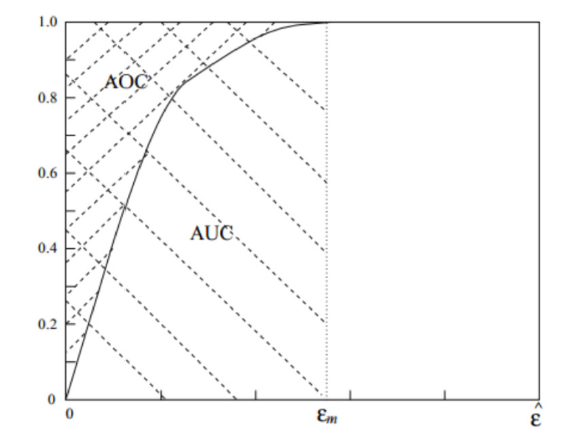
\includegraphics[width=0.7\linewidth]{REC-curve}
	\caption{Esempio di curva REC.}
	\label{fig:rec-curve}
\end{figure}
